\documentclass[convert={outfile=\jobname.svg}]{standalone}
\usepackage[dvipsnames]{xcolor}
\usepackage{tikz}
\tikzset{dot/.style={draw,shape=circle,fill=black,scale=0.4}}
\usepackage[outline]{contour}
\contourlength{0.05em}
\newcommand{\outline}[1]{\contour*{white}{#1}}

\begin{document}
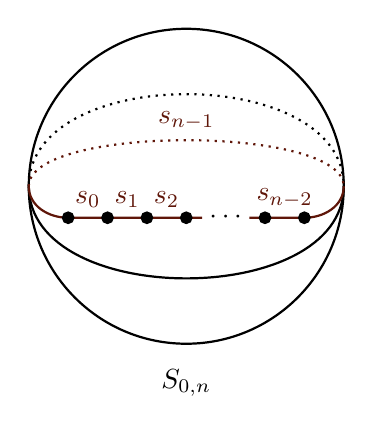
\begin{tikzpicture}[scale=2, thick]
    \draw (0, 0) circle (1);
    \draw (-1, 0) to [out=270,in=270] (1, 0);
    \draw [dotted] (-1, 0) to [out=90,in=90] (1, 0);
    
    \draw [Sepia, dotted] (-1, 0) to [out=90,in=90, looseness=0.5] node [above] {$s_{n-1}$} (1, 0);
    
    \draw [Sepia] (-1, 0)
        to [out=270,in=180] (-0.75, -0.2)
        to node [above] {$s_0$} (-0.5, -0.2)
        to node [above] {$s_1$} (-0.25, -0.2)
        to node [above] {$s_2$} (0, -0.2)
        to (0.1, -0.2);
    \node at (0.25, 0.-0.2) {$\cdots$};
    \draw [Sepia] (0.4, -0.2)
        to (0.5, -0.2)
        to node [above] {$s_{n-2}$} (0.75, -0.2)
        to [out=0,in=270] (1, 0);
    
    \node [dot] at (-0.75, -0.2) {};
    \node [dot] at (-0.5, -0.2) {};
    \node [dot] at (-0.25, -0.2) {};
    \node [dot] at (0, -0.2) {};
    \node at (0, -1.25) {$S_{0,n}$};
    \node [dot] at (0.5, -0.2) {};
    \node [dot] at (0.75, -0.2) {};
\end{tikzpicture}
\end{document}
